\section{ITS}
    ITS(Intelligent Transport Systems, 지능형 교통 체계)는 도로, 철도, 공항 등 교통 시설과 자동차, 열차 등 교통 수단 등 교통 체계 구성 요소에 전자, 통신, 제어 등 첨단기술을 접목하여 교통 체계의 운영 및 관리를 과학화, 자동화하고, 교통의 효율성과 안정성을 향상시키는 교통 체계이다. 차량번호 자동 인식, 실시간 신호 제어, 실시간 도로 교통 정보, 하이패스, 버스 도착 안내 시스템,  등이 ITS 서비스의 예시이다. ITS 구축을 통해 기존 도로의 이동 효율을 높이고 교통 혼잡 완화 및 교통 이용 편의 증진, 교통사고 예방, 교통안전성 향상, 교통체계의 효율적 운영 및 관리, 환경 보전 및 에너지 절감 등 다양한 효과를 기대할 수 있다. \\
    \vspace{-4mm}
    \begin{figure}[!h]\centering
		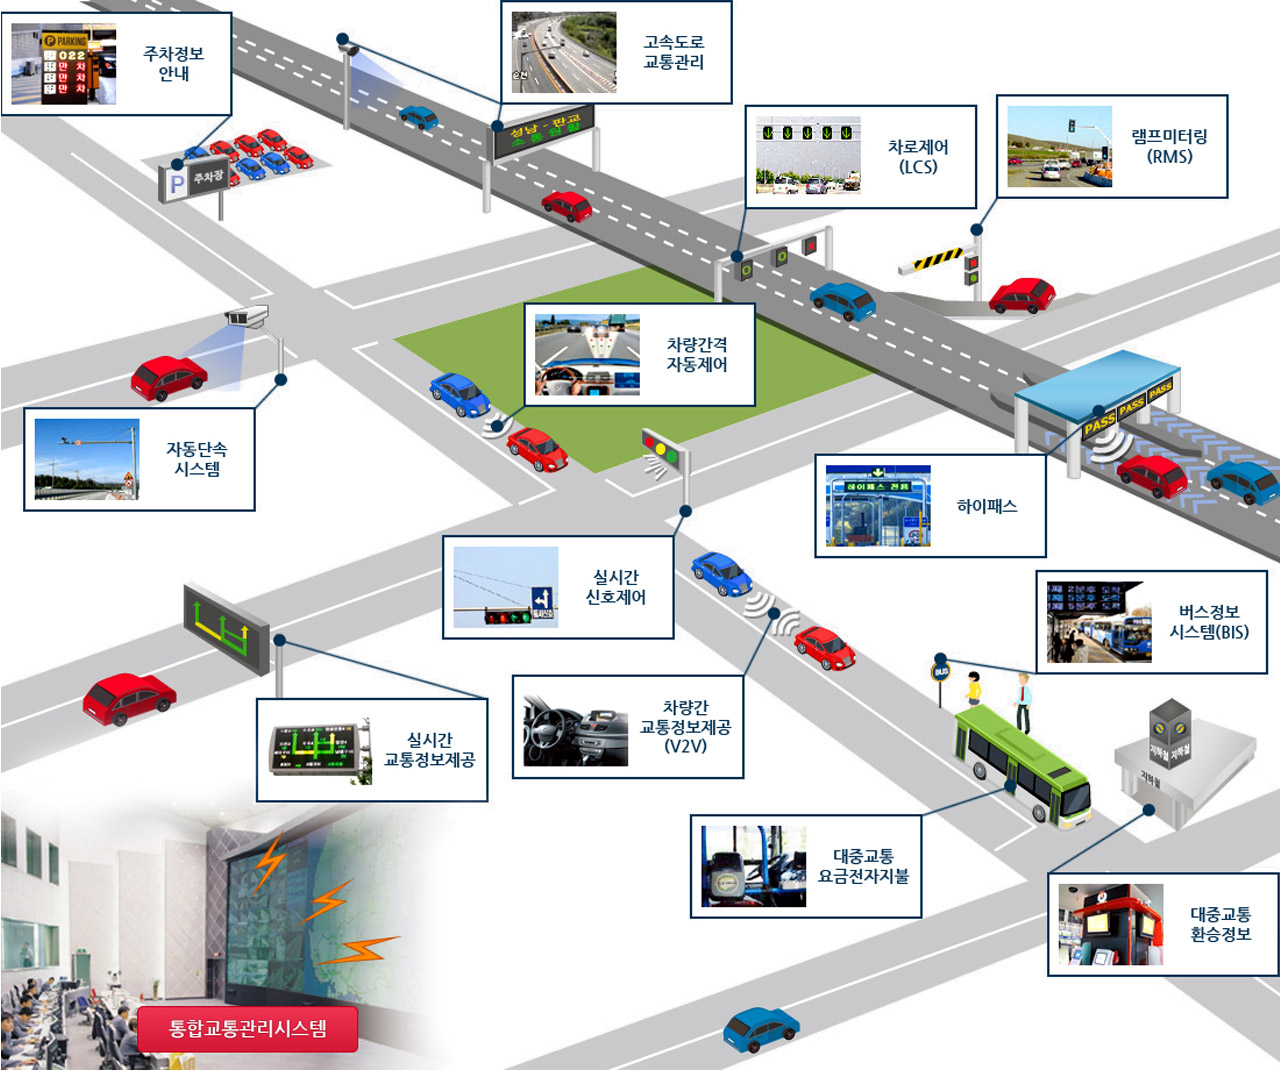
\includegraphics[width=.65\textwidth]{image/week13/1-1.png}
		\caption{\small ITS(지능형 교통 체계)}
		\vspace{-10pt}
    \end{figure}